\section{Experimentación}

En esta sección mostraremos los resultados de las pruebas con los distintos métodos de preprocesado de datos y modelos; con el objetivo de encontrar la combinación que nos dé los mejores resultados.

Antes de comentar específicamente los distintos métodos que probaremos, explicaremos la forma en la que se han realizado estas pruebas.

Como hemos comentado anteriormente, separamos los datos de entreno y prueba aplicando la opción de \textit{stratify} y con una proporción de \textit{75/25\%} respectivamente.

Una vez separados los conjuntos de datos, los tenemos que preprocesar. Para ello, hemos utilizado el objeto \textit{Pipeline} \cite{sklearnp32:online}, el cual nos permite encadenar diferentes pasos de preprocesado para entrenar diferentes modelos de forma sencilla. Por ejemplo, si queremos probar diferentes modelos, podemos hacerlo de la siguiente forma: 

\begin{enumerate}
    \item Instanciamos los objetos de las diferentes clases de preprocesado que queramos probar con sus respectivos valores. En el caso excepcional de la \textit{primera derivada}, hemos creado nuestro propio \textit{Transformer} (objeto de ``preprocesado'') que aplica la derivada a los datos.
    \item Los agregamos a la \textit{Pipeline} en orden.
    \item Ajustamos la \textit{Pipeline} sobre el conjunto de datos de entreno.
    \item Aplicamos la \textit{Pipeline} ya configurada sobre los datos de entreno y prueba. 
\end{enumerate}


El \textit{Pipeline} nos ofrece la ventaja de poder guardar y cargar tanto el orden del procedimiento, como la configuración de los pasos intermedios para aplicarlos más adelante de forma sencilla. Por ejemplo el \textit{StandardScaler}, para modificar los datos de forma que tengan media 0 y varianza 1, guarda la media y la varianza de cada columna para poder aplicarla más adelante.

Vale la pena comentar también que este objeto de \textit{Pipeline} nos ayuda a compartir la configuración del preprocesado entre la aplicación de entrenamiento de modelos y la de visualización de las predicciones sobre los archivos \gls{bil}.

Una vez hemos separado, preprocesado los datos y entrenado los modelos; para evaluar los modelos resultantes, hemos utilizado las métricas que hemos comentado en la \textit{Sección\ \ref*{sec:classification-metrics}} y además la \textit{Accuracy} sobre los datos de entreno como los de prueba, representados en las tablas por \textit{Test} y \textit{Train score}.
Dado que tenemos cuatro métricas, les hemos dado la siguiente preferencia:
\begin{enumerate}
    \item $Balanced\ Accuracy$
    \item $f2score$
    \item $\Delta Accuracy\ scores$: ($Train\ score-Test\ score$), utilizado 
\end{enumerate}


\subsection{Análisis del impacto de la primera derivada}

Para probar que, como hemos comentado antes, el aplicar la primera derivada sobre los datos nos puede ayudar a la hora de predecir, podemos comparar los resultados de entrenar con o sin derivar en la \textit{Tabla\ \ref{tab:nopreprocessing-derivative-results}}. En esta, podemos ver los resultados de entrenar la batería de modelos evaluados con las diferentes métricas que hemos comentado anteriormente. Vemos que, en general, la métrica que nos importa \textit{Balanced Accuracy} ha mejorado un \textbf{3.79\%}, por lo tanto, continuaremos aplicando la derivada en los siguientes pasos.

Además en la \textit{Tabla\ \ref{tab:nopreprocessing-derivative-results}} podemos ver un comportamiento que se repite, hay algunos modelos con un \textit{f2score} de \textit{0}, lo cual nos indica que el modelo no ha sido capaz de predecir correctamente la clase minoritaria. Esto también lo podemos ver en los modelos que su \textit{Balanced Accuracy} se acerca a $\frac{100}{n\_clases}$, en nuestro caso $50$, pues $n\_clases=2$.


\begin{table}[!ht]
    \centering
    \resizebox{\textwidth}{!}{\begin{tabular}{|c|cccc|cccc|}
        \hline
        & \multicolumn{4}{|c|}{Derivative} & \multicolumn{4}{c|}{No preprocessing} \\ \hline
        Model Name & Train score & Test score & f2score & Balanced accuracy & Train score & Test score & f2score & Balanced accuracy \\ \hline
        XGBoost & 82 & 82 & 0 & 50 & 82 & 82 & 0 & 50 \\ 
        Stochastic Gradient Descent & 18 & 18 & 52.326 & 50 & 18 & 18 & 52.326 & 50 \\ 
        Random Forest & 99.926 & 87.778 & 38.352 & 66.531 & 99.556 & 84.889 & 49.096 & 70.069 \\ 
        Quadratic Discriminant Analysis & 100 & 82 & 0 & 50 & 100 & 82 & 0 & 50 \\ 
        Multi-Layer Perceptron & 83.259 & 80.667 & 5.917 & 51.114 & 82 & 82 & 0 & 50 \\ 
        Linear Discriminant Analysis & 85.333 & 78.222 & 17.711 & 53.96 & 84.889 & 78 & 18.919 & 54.306 \\ 
        LightGBM & 81.852 & 72 & 59.794 & 71.846 & 75.778 & 64 & 48.708 & 62.632 \\ 
        K-Neighbors & 100 & 86.889 & 50.265 & 71.289 & 100 & 91.778 & 70.513 & 82.46 \\ 
        Hist Gradient Boosting & 78.444 & 70.444 & 55.785 & 68.97 & 72.815 & 63.556 & 42.77 & 58.988 \\ 
        Extra Trees & 99.63 & 90.444 & 63.802 & 78.756 & 94.667 & 81.111 & 63.636 & 76.438 \\ 
        Decision Tree & 56.963 & 58.889 & 58.244 & 67.224 & 82 & 82 & 0 & 50 \\ \hline
        \textit{Average} & ~ & ~ & ~ & \textbf{61.790} & ~ & ~ & ~ & 59.535 \\ \hline 
    \end{tabular}}
    \caption{Comparación de los resultados de entrenar utilizando la derivada y sin preprocesar. Fuente propia.}\ \label{tab:nopreprocessing-derivative-results}
\end{table}

\subsection{Análisis del impacto de aplicar la transformada}

Podemos ver los resultados de entrenar utilizando la transformada sobre los datos derivados en la \textit{Tabla\ \ref{tab:derivative-transformed-results}}, vemos que la métrica \textit{Balanced Accuracy} en general empeora en un \textbf{1.81\%}, así que continuaremos las pruebas sin añadir la transformada al preprocesado.

\begin{table}[!h]
    \centering
    \resizebox{\textwidth}{!}{\begin{tabular}{|c|cccc|cccc|}
        \hline
            & \multicolumn{4}{|c|}{Transformer and derivative} & \multicolumn{4}{c|}{Derivative} \\ \hline
            Model Name & Train score & Test score & f2score & Balanced accuracy & Train score & Test score & f2score & Balanced accuracy \\ \hline
        XGBoost & 82 & 82 & 0 & 50 & 82 & 82 & 0 & 50 \\ 
        Stochastic Gradient Descent & 18 & 18 & 52.326 & 50 & 18 & 18 & 52.326 & 50 \\ 
        Random Forest & 99.926 & 87.778 & 38.352 & 66.531 & 99.926 & 87.778 & 38.352 & 66.531 \\ 
        Quadratic Discriminant Analysis & 100 & 83.333 & 13.393 & \textbf{55.149} & 100 & 82 & 0 & 50 \\ 
        Multi-Layer Perceptron & 82 & 82 & 0 & 50 & 83.259 & 80.667 & 5.917 & 51.114 \\ 
        Linear Discriminant Analysis & 85.185 & 76.667 & 16.129 & 52.529 & 85.333 & 78.222 & 17.711 & 53.96 \\ 
        LightGBM & 81.852 & 72 & 59.794 & 71.846 & 81.852 & 72 & 59.794 & 71.846 \\ 
        K-Neighbors & 100 & 80.222 & 20.718 & \textbf{56.143} & 100 & 86.889 & 50.265 & 71.289 \\ 
        Hist Gradient Boosting & 78.444 & 70.444 & 55.785 & 68.97 & 78.444 & 70.444 & 55.785 & 68.97 \\ 
        Extra Trees & 99.63 & 90 & 64.433 & 78.967 & 99.63 & 90.444 & 63.802 & 78.756 \\ 
        Decision Tree & 56.963 & 58.889 & 58.244 & 67.224 & 56.963 & 58.889 & 58.244 & 67.224 \\ \hline
        \textit{Average} & ~ & ~ & ~ & 60.669 & ~ & ~ & ~ & \textbf{61.790} \\ \hline
        \end{tabular}}
    \caption{Comparación de los resultados de entrenar transformando y derivando los datos; frente a solo derivando. Fuente propia.}\ \label{tab:derivative-transformed-results}
\end{table}

\subsection{Estandarización}

Al aplicar la estandarización de los datos después de derivarlos obtenemos los resultados de la \textit{Tabla\ \ref{tab:derivative-standarization-results}}, los cuales en general son notablementes mejores que los anteriores, viendo una mejora del \textbf{4.43\%} en la \textit{Balanced Accuracy}. Estas mejoras ocurren en los modelos marcados en la tabla, \textit{QDA} y \textit{MLP}.


\begin{table}[!h]
    \resizebox{\textwidth}{!}{\begin{tabular}{|c|cccc|cccc|}
        \hline
        & \multicolumn{4}{c|}{Derivative + Scaler} & \multicolumn{4}{c|}{Derivative} \\ \hline
        Model Name & Train score & Test score & f2score & Balanced accuracy & Train score & Test score & f2score & Balanced accuracy \\ \hline
        XGBoost & 82 & 82 & 0 & 50 & 82 & 82 & 0 & 50 \\ 
        Stochastic Gradient Descent & 64.815 & 56.444 & 31.809 & 49.834 & 18 & 18 & 52.326 & 50 \\ 
        Random Forest & 99.926 & 87.778 & 38.352 & 66.531 & 99.926 & 87.778 & 38.352 & 66.531 \\ 
        Quadratic Discriminant Analysis & 96.148 & 83.111 & 55.012 & \textbf{72.358} & 100 & 82 & 0 & 50 \\ 
        Multi-Layer Perceptron & 90.815 & 84 & 24.355 & \textbf{59.41} & 83.259 & 80.667 & 5.917 & 51.114 \\ 
        Linear Discriminant Analysis & 85.333 & 78.222 & 17.711 & 53.96 & 85.333 & 78.222 & 17.711 & 53.96 \\ 
        LightGBM & 82.222 & 72.222 & 59.917 & 71.981 & 81.852 & 72 & 59.794 & 71.846 \\ 
        K-Neighbors & 100 & 86.889 & 49.202 & 70.807 & 100 & 86.889 & 50.265 & 71.289 \\ 
        Hist Gradient Boosting & 78.444 & 70.444 & 55.785 & 68.97 & 78.444 & 70.444 & 55.785 & 68.97 \\ 
        Extra Trees & 99.63 & 90.444 & 63.802 & 78.756 & 99.63 & 90.444 & 63.802 & 78.756 \\ 
        Decision Tree & 56.963 & 58.889 & 58.244 & 67.224 & 56.963 & 58.889 & 58.244 & 67.224 \\ \hline
        \textit{Average} & ~ & ~ & ~ & \textbf{64.530} & ~ & ~ & ~ & 61.790 \\ \hline
        \end{tabular}}
    \caption{Comparación de los resultados de entrenar derivando y estandarizando los datos; frente a solo derivando. Fuente propia.}\ \label{tab:derivative-standarization-results}
\end{table}


\subsection{Aumento y disminución de dimensionalidad}


Por último, aun siendo un paso generalmente recomendado, el aumento y disminución de dimensionalidad nos ha dado los resultados de la \textit{Tabla\ \ref{tab:derivative-standarization-dimensionality-results}}, los cuales son significativamente peores que los anteriores empeorando la \textit{Balanced Accuracy} en un \textbf{5.66\%}. Por lo tanto, continuaremos con los datos derivados y estandarizados sin aumentar o disminuir la dimensionalidad de los datos.

\begin{table}[!h]
    \resizebox{\textwidth}{!}{\begin{tabular}{|c|cccc|cccc|}
        \hline
            & \multicolumn{4}{c|}{Derivative + Scaler + Polynomial Features + PCA} & \multicolumn{4}{c|}{Derivative + Scaler} \\ \hline
            Model Name & Train score & Test score & f2score & Balanced accuracy & Train score & Test score & f2score & Balanced accuracy \\ \hline
        XGBoost & 82 & 82 & 0 & 50 & 82 & 82 & 0 & 50 \\ 
        Stochastic Gradient Descent & 53.333 & 50.444 & 40.468 & 52.439 & 64.815 & 56.444 & 31.809 & 49.834 \\ 
        Random Forest & 99.926 & 85.778 & 28.818 & 61.939 & 99.926 & 87.778 & 38.352 & 66.531 \\ 
        Quadratic Discriminant Analysis & 80.889 & 80 & 38.168 & \textbf{63.234} & 96.148 & 83.111 & 55.012 & \textbf{72.358} \\ 
        Multi-Layer Perceptron & 87.778 & 81.778 & 14.493 & 54.682 & 90.815 & 84 & 24.355 & 59.41 \\ 
        Linear Discriminant Analysis & 82.741 & 81.111 & 4.491 & 50.903 & 85.333 & 78.222 & 17.711 & 53.96 \\ 
        LightGBM & 77.037 & 68.444 & 46.512 & \textbf{62.933} & 82.222 & 72.222 & 59.917 & \textbf{71.981} \\ 
        K-Neighbors & 100 & 83.778 & 36.486 & \textbf{64.092} & 100 & 86.889 & 49.202 & \textbf{70.807} \\ 
        Hist Gradient Boosting & 75.63 & 66 & 46.296 & 61.924 & 78.444 & 70.444 & 55.785 & 68.97 \\ 
        Extra Trees & 96.222 & 82.222 & 51.597 & 70.37 & 99.63 & 90.444 & 63.802 & 78.756 \\ 
        Decision Tree & 71.852 & 68.889 & 30.892 & \textbf{55.014} & 56.963 & 58.889 & 58.244 & \textbf{67.224} \\ \hline
        \textit{Average} & ~ & ~ & ~ & \textbf{58.866} & ~ & ~ & ~ & \textbf{64.530} \\ \hline
        \end{tabular}} 
    \caption{Comparación de los resultados de entrenar derivando, estandarizando y ajustando la dimensionalidad de los datos; frente a solo derivando y estandarizando. Fuente propia.}\ \label{tab:derivative-standarization-dimensionality-results}
\end{table}


\subsection{Selección de modelos y \textit{hyperparameter tuning}}\ \label{sec:entrenamiento}

Una vez encontrada una combinación de pasos de preprocesado que nos mejora los resultados, podemos pasar al siguiente paso de selección de los modelos. Habiendo entrenado ya los modelos, vemos que algunos hacen \textit{overfitting}. El \textit{overfitting} ocurre cuando un modelo se ajusta demasiado a los datos con los que ha entrenado y no generaliza bien, es decir que predice mejor los datos con los que ha entrenado que datos nuevos. Donde lo podemos ver más claramente es en \textit{KNeighbors}, vemos en la \textit{Figura\ \ref{fig:lc-knn}} que, para cualquier cantidad de datos con los que entrenemos el modelo, siempre predecirá bien con los que ha entrenado y no tanto con los demás. Nuestro objetivo es intentar que ambos valores no sean tan dispares y que sean lo más altos posibles, para ello haremos \textit{hyperparameter tuning}.

\begin{figure}[!h]
    \centering
    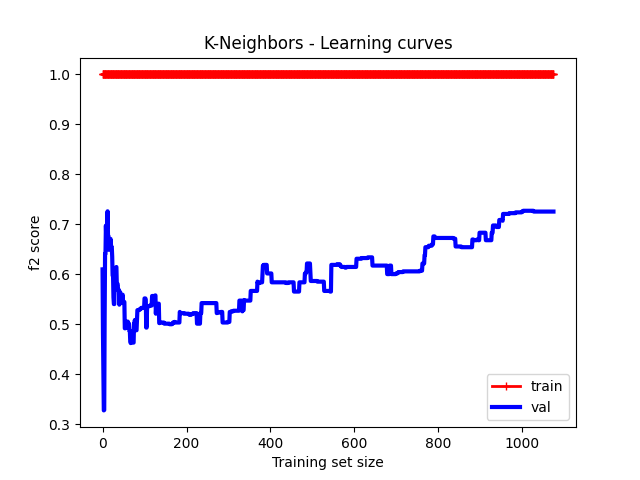
\includegraphics[width=0.7\linewidth]{media/images/learing-curves-knn.png}
    \caption{Gráfico de la curva de aprendizaje del modelo \textit{K-Neighbors} entrenándolo y probándolo sobre los datos de entreno únicamente. Fuente propia}\ \label{fig:lc-knn}
\end{figure}

Para evitar el \textit{overfitting}, uno de los posibles remedios es utilizar \textit{hyperparameter tuning}. El \textit{hyperparameter tuning} tiene como objetivo encontrar un conjunto de parámetros que maximice el rendimiento del modelo sobre los datos de prueba. En nuestro caso, como los datos están desbalanceados, podemos utilizar como función de rendimiento el \textit{balanced accuracy}. Como cada modelo es distinto, debemos encontrar los parámetros adecuados para cada uno. 

Para ahorrarnos tiempo podemos utilizar solamente los mejores modelos, como hemos visto en los resultados de la \textit{Tabla\ \ref{tab:derivative-standarization-dimensionality-results}}, hay modelos que tienen mejores resultados que otros. Así que escogeremos los cuatro con mejor \textit{balanced accuracy}, es decir: \textit{Extra Trees, Quadratic Discriminant Analysis, LightGBM y K-Neighbors}.

Realizaremos el \textit{hyperparameter tuning} en dos pasos, primeramente utilizaremos \textit{Random Search} y después \textit{Grid Search}, ya implementados en \textit{sklearn}.
Ambos métodos utilizan \textit{cross-validation}, una técnica para evitar el \textit{overfitting} que consiste en la división de los datos de entreno en partes iguales.
Una vez dividido en \textit{N} partes, se entrena el modelo sobre todas las partes excepto una, la cual se utiliza para evaluar el modelo entrenado. Entonces, se repite el 
proceso cambiando de partición. De esta forma, haciendo la media obtenemos el resultado de entrenar el modelo repetidas ocasiones con los mismos parámetros, pero con datos 
distintos. Una vez hemos obtenido el mejor de los modelos que hemos entrenado, según la función de rendimiento, probamos el modelo resultante sobre los datos de prueba.
Podemos ver este proceso más gráficamente en la \textit{Figura\ \ref{fig:cross-validation}}.

\begin{figure}[!h]
    \centering
    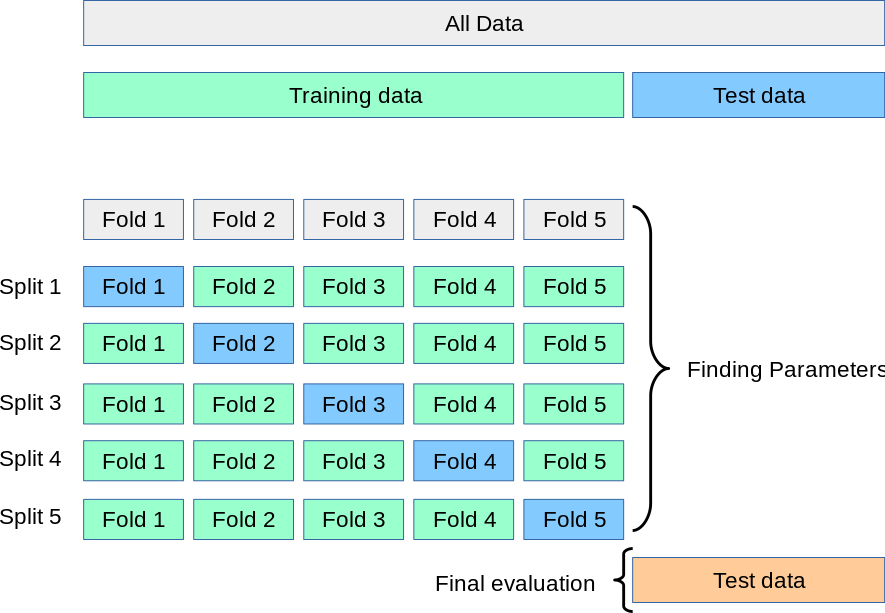
\includegraphics[width=0.7\linewidth]{media/images/cross-validation.png}
    \caption{\textit{Cross-validation} explicado gráficamente. Fuente:\ \cite{31Crossv20:online}}\ \label{fig:cross-validation}
\end{figure}


El \textit{random search} consiste en la búsqueda de estos parámetros habiendo definido un rango de posibilidades. Es decir, para cada parámetro que le queramos
pasar al modelo definiremos un rango de valores que puede tener, entonces el \textit{random search} entrena el modelo repetidas veces con una permutación aleatoria de sus 
parámetros y se guarda los resultados. Podemos ver un ejemplo en el \textit{Código\ \ref{code:random-search-example}}.
Podemos ir probando diferentes parámetros y rangos hasta que estemos satisfechos con el resultado.


Una vez estemos contentos con los resultados, los refinaremos utilizando \textit{grid search}. A diferencia del \textit{random search}, el \textit{grid search} prueba todas
las posibles combinaciones que le pasemos como parámetro y, consecuentemente, es mucho más lento. Por ello, utilizaremos el \textit{grid search} con los mejores parámetros que
encontremos del paso anterior, los cuales son potencialmente los mejores. Una vez definido un rango de parámetros para los modelos seleccionados, obtenemos los resultados
de la \textit{Tabla\ \ref{tab:hyperparameter-tuning-results}}. Podemos ver que hemos obtenido, en general, peores resultados (salvo con \textit{K-Neighbors}), por lo tanto
deberíamos ajustar el rango de parámetros que les pasamos a los modelos y volver a entrenarlos hasta que estemos satisfechos con el resultado. En nuestro caso no lo haremos
y pasaremos a la segunda iteración del proyecto para probar nuevas cosas en pasos anteriores.

\begin{table}[!h]
    \centering
    \begin{tabular}{|c|cccc|}
        \hline
        Model name & Train score & Test score & f2 score & Balanced accuracy \\ \hline
        RS - knn & 100 & 90.274 & 83.96 & 90.274 \\
        GS - knn & 100 & 90.274 & 83.96 & 90.274 \\
        RS - qda & 97.491 & 72.358 & 55.012 & 72.358 \\
        GS - qda & 97.491 & 72.358 & 55.012 & 72.358 \\
        RS - lgbm & 86.013 & 71.018 & 58.333 & 71.018 \\
        GS - et & 82.957 & 66.17 & 47.945 & 66.17 \\
        GS - lgbm & 84.628 & 70.626 & 58.704 & 70.626 \\
        RS - et & 69.492 & 65.854 & 53.254 & 65.854 \\ \hline
        \end{tabular}
    
    \caption{Resultados del primer entrenamiento con hyperparameter tuning. Fuente propia.}\ \label{tab:hyperparameter-tuning-results}
\end{table}
\clearpage

\subsection{Balanceo de datos}\ \label{sec:i2-balance}

\subsubsection{\textit{Undersampling}}

Al probar los algoritmos mencionados anteriormente, obtenemos los resultados de la \textit{Tabla\ \ref{tab:undersampling-methods}}. 
Hemos agregado una columna más, \textit{Avg. score diff}, que nos indica la diferencia entre el \textit{Train} y \textit{Test score} para decidir mejor, pues las demás métricas nos daban resultados bastante parecidos. Esta ``nueva'' métrica no indica cuánto \textit{overfitting} hacen los modelos que se entrenan sobre el dataset generado, por lo tanto, cuanto más cercana a \textit{0} sea, mejor. Podemos ver que, en general, los diferentes \textit{Near Miss}, obtienen resultados bastante peores que los otros métodos. En cuanto a los otros tres algoritmos restantes, podemos ver que el \textit{Tomek Links} es el que mejores resultados tiene, así que continuaremos utilizándolo.

Podemos ver en la \textit{Figura\ \ref{fig:balance-tl}} la comparación del balance de la clase objetivo antes y después de utilizar el método \textit{Tomek Links}. Para hacer la comparación hemos tenido en cuenta que los modelos resultantes hicieran el menor \textit{overfitting} posible utilizando el \textit{Avg. score diff} el cual es la diferencia entre el \textit{Train} y \textit{Test score}. También hemos tenido en cuenta que las métricas \textit{f2 score} y \textit{balanced accuracy} fueran lo más altas posibles. Podemos ver que, aunque no ha mejorado mucho el balance de las clases (como nos muestra la \textit{Tabla\ \ref{tab:balance-tl-comparison}})), los resultados son mejores que sin utilizar ningún método de balanceo.

\begin{table}[!ht]
    \centering
    \begin{tabular}{|c|ccc|} \hline
        & Avg. score diff & Avg. f2 Score & Avg. Balanced Accuracy \\ \hline
        \textit{NM v1} & 35.263 & 53.698 & 62.754 \\
        \textit{NM v2} & 41.914 & 53.592 & 61.315 \\
        \textit{NM v3} & 9.883 & 39.654 & 61.999 \\
        \textit{RUS} & 9.176 & 41.954 & 63.656 \\
        \textit{ENN (ALL)} & 10.410 & 46.600 & 66.523 \\
        \textit{ENN (MODE)} & 8.953 & 42.018 & 64.575 \\
        \textit{TL} & 7.950 & 42.610 & 65.236 \\ \hline
    \end{tabular}
    \caption{Resultado de entrenar los modelos básicos sobre el \textit{dataset} reducido con los diferentes métodos. Fuente: propia.}\ \label{tab:undersampling-methods}
\end{table}

\begin{figure}[!ht]
    \centering
    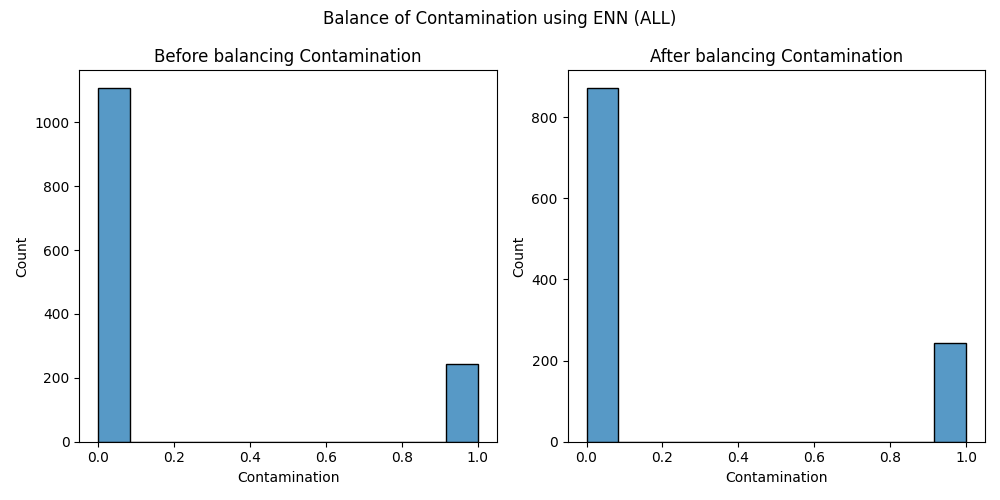
\includegraphics[width=0.8\linewidth]{media/images/balance.png}
    \caption{Comparación del balance de la clase objetivo antes y después de utilizar el método de \textit{undersampling ENN (ALL)}. Fuente propia.}\ \label{fig:balance-tl}
\end{figure}

\begin{table}
    \centering
    \begin{tabular}{|c|cc|} \hline
        & Good samples & Bad samples \\ \hline
        Before undersampling & 1107 & 243 \\
        After undersampling & 1095 & 243 \\ \hline
    \end{tabular}
    \caption{Comparación de las muestras antes y después de aplicar \textit{Tomek Links}. Fuente propia.}\ \label{tab:balance-tl-comparison}
\end{table}


\clearpage

\subsubsection{\textit{Oversampling}}

Antes de comentar los sintetizadores que probaremos, definiremos el método con los que evaluaremos los datos generados. Para ello utilizaremos una función de la propia librería \textit{sdv} que evalúa la similitud estadística de los datos generados con los datos reales y nos genera un \textit{quality report}.

Una vez hemos entrenado los sintetizadores, evaluamos su similitud con los datos reales y obtenemos los resultados de la \textit{Tabla\ \ref{tab:oversampling-quality-report}}, en los cuales podemos ver un claro `ganador'.

\begin{table}[!ht]
    \centering
    \resizebox{0.8\linewidth}{!}{\begin{tabular}{|c|ccc|} \hline
        Synthesizer & Column Shapes & Column Pair Trends & Overall Quality \\ \hline
        Gaussian Copula Synthesizer & 94.75 & 99.83 & 97.29 \\
        TVAE Synthesizer & 84.37 & 74.97 & 79.64 \\ \hline
    \end{tabular}}
    \caption{Resultados del \textit{quality report} de los datos generados con los sintetizadores. Fuente propia}\ \label{tab:oversampling-quality-report}
\end{table}

Ahora que tenemos el sintetizador que mejores resultados nos da, lo aplicamos sobre la clase minoritaria y generamos datos sintéticos. Una vez generados, entrenamos los modelos básicos y obtenemos los resultados de la \textit{Tabla\ \ref{tab:balanced-basic-training}}. Podemos ver que, en general, los modelos resultantes son peores que los que se han entrenado con datos que no utilizan ningún sintetizador, por lo tanto, mantendremos el \textit{undersampling}, pero no utilizaremos \textit{oversampling} en los siguientes pasos.


\begin{table}[!ht]
    \centering
    \resizebox{\textwidth}{!}{\begin{tabular}{|c|cccc|}\hline
        Model Name & Train score & Test score & f2score & Balanced accuracy \\ \hline
        XGBoost & 89.908 & 78.889 & 21.622 & 55.812 \\ 
        Stochastic Gradient Descent & 79.53 & 69.333 & 27.972 & 53.839 \\ 
        Random Forest & 97.42 & 82.444 & 42.526 & 66.17 \\ 
        Quadratic Discriminant Analysis & 93.005 & 82.667 & 10.448 & 53.779 \\ 
        Multi-Layer Perceptron & 94.209 & 80.889 & 40.712 & 64.74 \\ 
        Linear Discriminant Analysis & 87.041 & 76.889 & 18.667 & 53.628 \\ 
        LightGBM & 90.195 & 77.111 & 14.946 & 52.319 \\ 
        K-Neighbors & 100 & 85.778 & 61.425 & 76.393 \\ 
        Hist Gradient Boosting & 86.812 & 77.333 & 16.26 & 52.936 \\ 
        Extra Trees & 90.998 & 80 & 25.606 & 57.934 \\ 
        Decision Tree & 83.658 & 80.222 & 7.31 & 51.325 \\ \hline
        Average & ~ & ~ & 26.135 & 58.079 \\ \hline
        \end{tabular}}
    \caption{Resultados de entrenar los modelos básicos habiendo balanceado el \textit{dataset}. Fuente propia.}\ \label{tab:balanced-basic-training}
\end{table}

\clearpage
\subsection{Nuevos modelos}

Hay dos tipos de modelos más complejos que no hemos probado que pueden darnos mejores resultados, estos son \textit{Voting Classifier} y \textit{Bagging Classifier}. El primero, \textit{Voting Classifier}, entrena los modelos que lo componen sobre el \textit{dataset} y, a la hora de predecir, extrapola su predicción en base a las predicciones de estos modelos. Es decir, realiza una votación y la clase que más se vote es la que sale como predicción como podemos ver en la \textit{Figura\ \ref{fig:voting-classifiers}}. Hay dos tipos de votación, \textit{hard} y \textit{soft}, \textit{hard} utiliza la clase predicha de los modelos, mientras que \textit{soft} suma las probabilidades de las clases a predecir y suele ser más preciso \cite{Ensemble96:online}. 

\begin{figure}[!h]
    \centering
    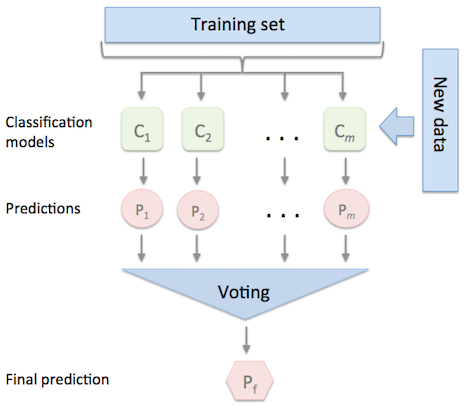
\includegraphics[width=0.7\linewidth]{media/images/majority_voting.png}
    \caption{Explicación gráfica del proceso de entreno y predicción de un \textit{Voting Classifier}. Fuente \cite{Ensemble96:online}.}\ \label{fig:voting-classifiers}
\end{figure}

Por otro lado \textit{Bagging Classifier} entrena el mismo modelo sobre un subconjunto aleatorio del \textit{dataset} y luego agrega los resultados de las predicciones, ya sea haciendo la media o realizando una votación, para obtener una predicción final.\ \cite{sklearne53:online}


Antes de entrenar estos modelos, hemos de decidir qué otros modelos los compondran, por lo tanto, escogeremos los que han tenido mejores resultados al entrenarlos sobre el \textit{dataset} balanceado. Estos son los que mejores resultados tienen en la \textit{Tabla\ \ref{tab:balanced-basic-training}}, es decir, \textit{K-Neighbors}, \textit{Multi-Layer Perceptron}, \textit{Random Forest} y \textit{Extra Trees}.

Al entrenar los \textit{Voting} y \textit{Bagging Classifiers}, obtenemos los resultados de la \textit{Tabla\ \ref{tab:voting-bagging-results}}. En general, los \textit{Voting} han obtenido resultados algo mejores que los \textit{Bagging Classifiers}, podría ser por la cantidad de datos sobre los que ha entrenado cada submodelo. De todas formas, en general, obtenemos mejores resultados que utilizando modelos básicos.

\begin{table}[!ht]
    \centering
    \resizebox{\textwidth}{!}{\begin{tabular}{|c|cccc|cccc|}    \hline
        & \multicolumn{4}{|c|}{Balanced dataset} & \multicolumn{4}{c|}{Normal dataset} \\ \hline
        Model Name & Train score & Test score & f2score & Balanced accuracy & Train score & Test score & f2score & Balanced accuracy \\ \hline
        Voting (RF, ET, KNN) & 100 & 87.111 & 39.216 & 66.606 & 100 & 86.889 & 40.278 & 66.953 \\
        Voting (MLP, ET) & 100 & 90.444 & 60.847 & 77.311 & 100 & 89.333 & 58.047 & 75.67 \\
        Voting (KNN, ET) & 99.402 & 87.111 & 47.17 & 69.979 & 99.111 & 86.667 & 46.917 & 69.708 \\
        Voting (KNN, ET) & 100 & 87.556 & 44.077 & 68.805 & 100 & 87.333 & 42.818 & 68.187 \\
        Bagging (RF) & 87.145 & 82.667 & 6.079 & 52.334 & 86.889 & 82 & 3.049 & 50.964 \\
        Bagging (MLP) & 91.031 & 82.667 & 18.732 & 56.67 & 90.741 & 83.111 & 17.493 & 56.459 \\
        Bagging (KNN) & 83.931 & 83.333 & 11.976 & 54.667 & 83.407 & 83.111 & 9.063 & 53.568 \\
        Bagging (ET) & 93.946 & 84.222 & 16.369 & 56.655 & 93.259 & 82.889 & 10.479 & 53.914 \\ \hline
        \end{tabular}
        }
        \caption{Resultados de entrenar los diferentes \textit{Voting} y \textit{Bagging Classifiers} que hemos preparado con los resultados del \textit{hyperparameter tuning}. Fuente propia.}\ \label{tab:voting-bagging-results}
\end{table}

\subsubsection{Hyperparameter tuning}

Además de los nuevos modelos, podemos volver a probar a hacer \textit{hyperparameter tuning} sobre el dataset balanceado, obteniendo los resultados de la \textit{Tabla\ \ref{tab:hyperparameter-tuning-results-v2}} que, compárandolos con los resultados del anterior \textit{hyperparameter tuning}, vemos que han mejorado un poco en general, por lo que eligiríamos estos últimos para predecir. 

\begin{table}[!ht]
    \centering
    \begin{tabular}{|c|cccc|} \hline
        Model name & Train score & Test score & f2 score & Balanced accuracy \\ \hline
        RS - knn & 100 & 91.509 & 86.035 & 91.509 \\
        GS - knn & 100 & 91.509 & 86.035 & 91.509 \\
        RS - qda & 97.694 & 72.282 & 54.455 & 72.282 \\
        GS - qda & 97.694 & 72.282 & 54.455 & 72.282 \\
        GS - lgbm & 85.107 & 71.304 & 59.305 & 71.304 \\
        RS - lgbm & 85.748 & 69.798 & 57.26 & 69.798 \\
        RS - et & 50 & 50 & 52.326 & 50 \\
        GS - et & 50 & 50 & 52.326 & 50 \\ \hline
    \end{tabular}
    \caption{Resultado del \textit{hyperparameter tuning} con el \textit{dataset} balanceado. Fuente propia.}\ \label{tab:hyperparameter-tuning-results-v2}
\end{table}